\chapter{}
\section{Details on the pair-production algorithm}
\label{sec:pairprod-appendixA}

Since this is the first implementation of the self-consistent pair production in a particle-in-cell code, in this Appendix we present the details about the algorithm we used in our simulations.

\begin{figure}[htb]
    \centering
    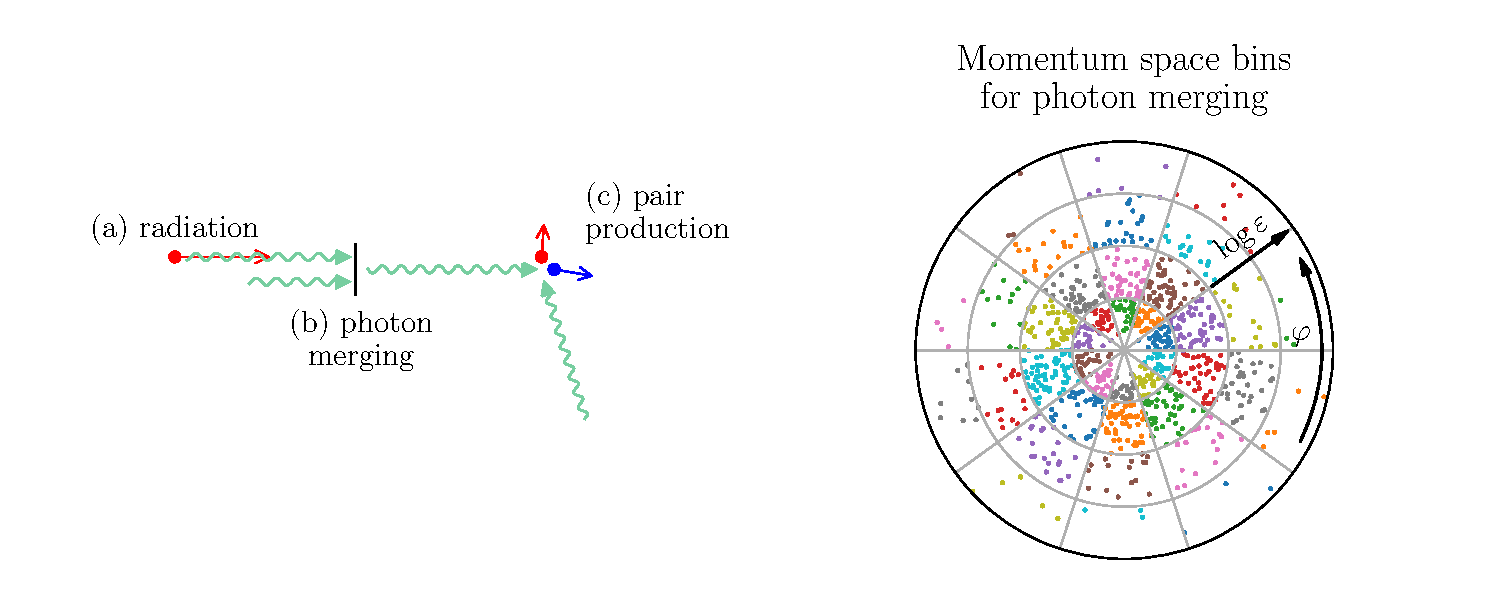
\includegraphics[width=.8\textwidth]{figures/ch4-pairproduction/fig_a1.pdf}
    \caption{{\it Left}: three main steps in our algorithm -- plasma particle radiation a photon, photons merging (downsampling) in a given cell, photons interacting and producing secondary pairs. {\it Right}: two-dimensional version of the momentum binning we use for the photon downsampling. Binning is logarithmic in energy (momentum magnitude) and uniform in direction. Photons are colored according to their location in those bins, all the photons of the same color will be merged into two photons with higher weights conserving energy and momenta.}
    \label{fig:pairprod-alg_scheme}
\end{figure}

We track two particle species: charged and massive plasma particles and massless photons. At each timestep a plasma particle can radiate a photon (step (a) in Figure~\ref{fig:pairprod-alg_scheme}, {\it left}) with a corresponding synchrotron energy given by formula (\ref{eq:pairprod-synch_form}), and the overall cooling rate is set by relation (\ref{eq:pairprod-synch_rate}). The photons are then resorted in memory according to their spatial location.

Since we intend to study the optically thin regime to pair production, $\tau_{\gamma\gamma}\ll1$, and at the same time we have a sufficiently high multiplicity of secondary pairs, in our simulations the typical number of photons greatly exceeds the number of particles. This can very quickly exhaust the memory capabilities. To avoid this we use a downsampling (merging) algorithm for the photons similar to one described by \cite{2015CoPhC.191...65V}.

In each simulation cell we define three-dimensional photon momentum bins and sort photons according to their momenta as seen in Figure~\ref{fig:pairprod-alg_scheme}, {\it right}. The bins are logarithmic in photon energies and uniform in 3D directions. We also randomly ``rotate'' the bins to minimize any downsampling artifacts. All the photons in the same momentum bin are then merged into two photons with higher effective weights (step (b) in Figure~\ref{fig:pairprod-alg_scheme}, {\it left}), conserving total energy and momentum. Note also, that since the downsampling is done for the lowest energy photons (which are the majority) and for those who have small relative momenta angles, downsampling does not strongly affect the pair production efficiency, since those photons have a negligible probability to pair produce.

Two-photon pair production (step (c) in Figure~\ref{fig:pairprod-alg_scheme}, {\it left}) is another expensive step that we implement in our simulation. At each cell we loop through all the non-repetitive pairs of photons and compute their binary probabilities $p_{ij}$ to pair produce given their energies, momenta and the cross section formula.

Since the weights of those photons can be greater than one, these probabilities as well can exceed unity, i.e., if $p_{ij}=4.2$ on average from these photons $i$ and $j$ we will create $4.2$ $e^-e^+$ pairs: $4$ pairs with a probability $1$ and one more pair with a probability $0.2$ (reducing the photon weights each time). This approach is designed to mimic as if these interactions were between independent photons not merged into a two ``heavy'' ones.

The probability magnitudes are normalized to a fiducial parameter, $p_0$, which is chosen to ensure the low optical depth to pair production. Overall the optical depth for a photon can be written as
\begin{equation}
    \tau_{\gamma\gamma} = L\langle n_{\rm ph}\rangle f_0 p_0,
\end{equation}
where $L$ is the effective size of the system, $\langle n_{\rm ph}\rangle$ is the average number of (potentially pair producing) photons per cell along the path, $p_0$ is our fiducial parameter, and the prefactor $f_0$ accounts for the cross section for different energies and momenta orientation (see Figure~\ref{fig:pairprod-sigma_pp}) and is typically $0.1\text{-}0.01$. In our simulations the size of the system is typically a few times $10^3$ cells, and the effective number of pair producing photons along the path can vary $10^2\text{-}10^3$ (less than the total number of photons per cell). This gives us a rough estimate that
\begin{equation}
    \tau_{\gamma\gamma} \sim \frac{p_0}{10^{-3}}.
\end{equation}

The difference between optically thick and thin regimes is demonstrated in Figure~\ref{fig:pairprod-opt_thick}. The evolution of a single photon generation spectra are different in these two cases ($p_0=10^{-3}$ and $p_0=10^{-5}$). In optically thick regime (Figure~\ref{fig:pairprod-opt_thick}, {\it right}) most of the high energy photons interact with lower energy ones and pair produce in less than a single light-crossing time, resulting in a lower cutoff energy, whereas in optically thin regime (Figure~\ref{fig:pairprod-opt_thick}, {\it left}) the spectrum nearly uniformly drops down over all energies due to pair production in a few light-crossing times.

\begin{figure}[htb]
    \centering
    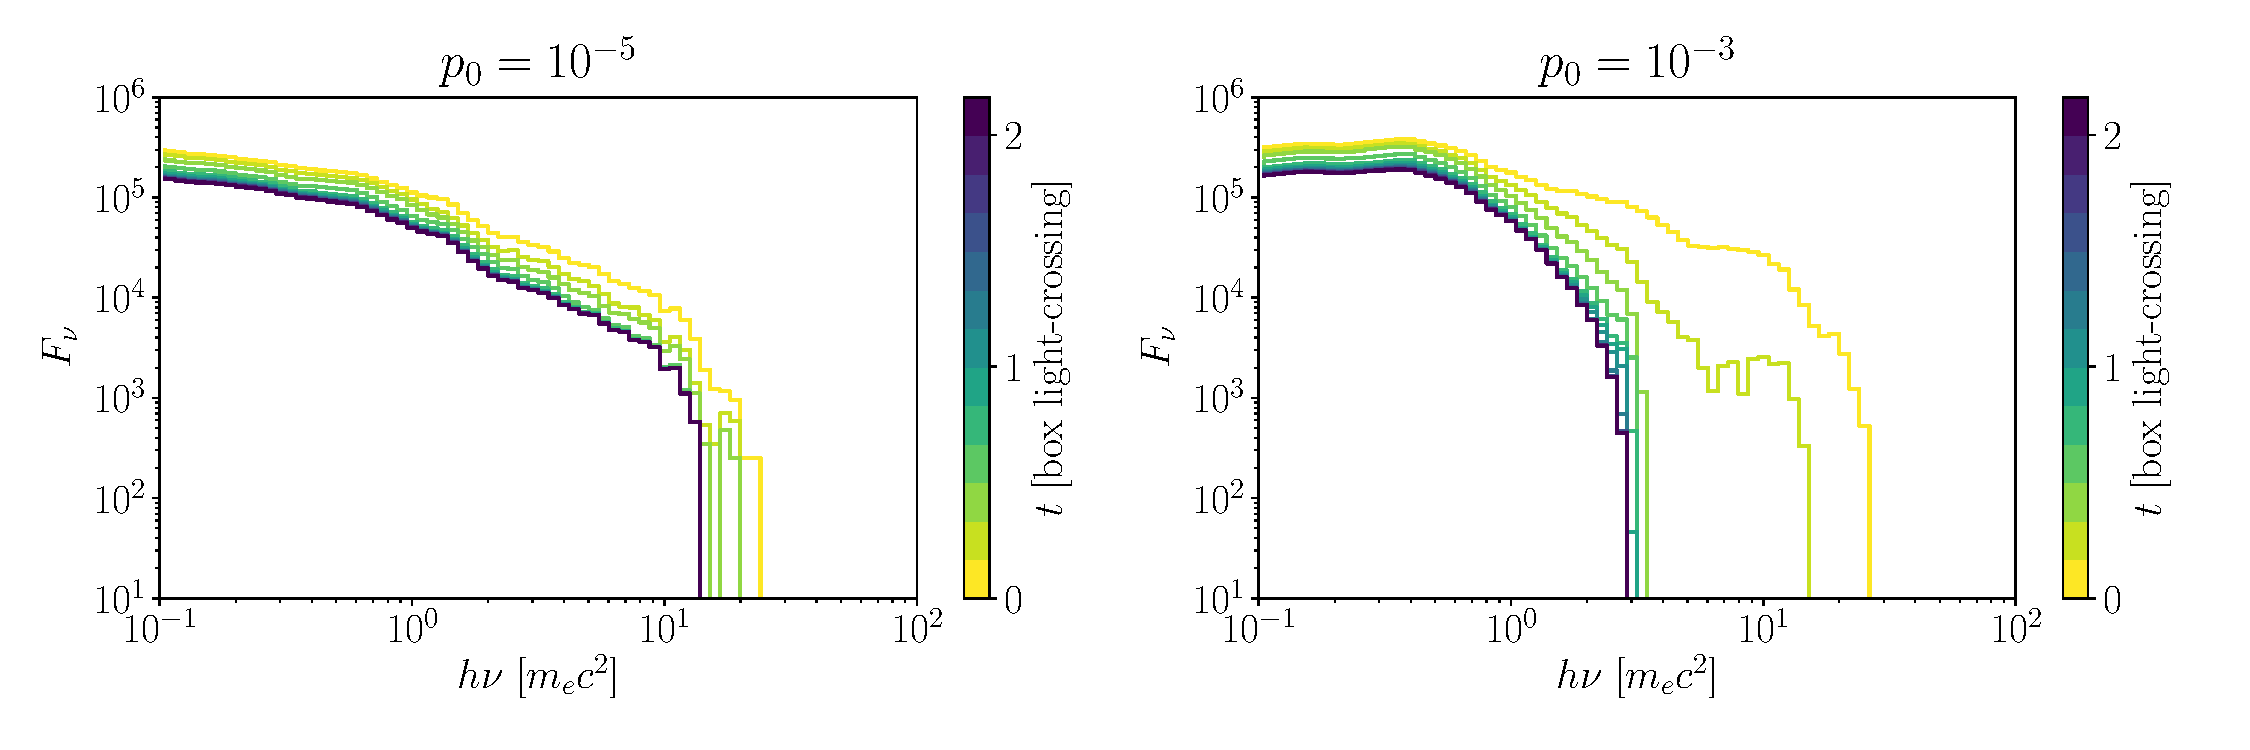
\includegraphics[width=.8\textwidth]{figures/ch4-pairproduction/fig_a2.pdf}
    \caption{Time evolution of the spectrum of photons born at the same timestep. The time is measured in box light-crossing times, {\it left} plot corresponds to an optically thin regime with $p_0=10^{-5}$, and {\it right} -- optically thick with $p_0=10^{-3}$. Spectra are corrected to photons leaving the box, i.e., the reduction is only due to pair production. In optically thick regime most of the high energy photons interact in less than a light-crossing time.}
    \label{fig:pairprod-opt_thick}
\end{figure}

\begin{table}
\begin{centering}
 \begin{tabular}{ l || c | c }
 \hline
  & Computational cost & Memory usage \\ [0.5ex]
 \hline\hline
 photon sorting & $\mathcal{O}(N_{\rm ph})$ & $\mathcal{O}(N_{\rm ph})$ \\
 photon merging & $\mathcal{O}(N_{\rm ph})$ & $\mathcal{O}(n_{\rm ph})$ \\
 pair production & $\mathcal{O}(n_{\rm ph} N_{\rm ph})$ & $\mathcal{O}(N_{\rm ph})$ \\ [1ex]
 \hline
\end{tabular}
\caption{Time and memory costs for the most expensive parts of our algorithm as a function of the total number of photson in the box, $N_{\rm ph}$, and the average number of photons in each cell, $n_{\rm ph}$. }
\label{table:comp}
\end{centering}
\end{table}

Finally, in Tab.~\ref{table:comp} we present the time and memory consumption of our algorithm as a function of the total number of photons, $N_{\rm ph}$, and the average number of photons per simulation cell, $n_{\rm ph}$. Pair production is the most expensive procedure, since it is $\sim\mathcal{O}(n_{\rm ph}^2 N_{\rm cells}) \sim \mathcal{O}(n_{\rm ph} N_{\rm ph})$.

Merging is efficient as far as the average number of photons per cell is $n_{\rm ph}\gg N_{\rm bins}$, where the number of momentum bins we typically use is $N_{\rm bins}=8^3=512$. In our typical run we have $10^4\text{-}10^5$ photons per cell, and, thus, this downsampling significantly decreases the cost by reducing the number of tracked photons typically by a factor of $10\text{-}100$.

In most of our runs this is still expensive, and we do this procedure once every several steps, instead of doing it every step. One, however, should keep in mind, that this interval cannot be longer than the typical mean free path of the photons to pair production (which in our case is a fraction of the box size), and also the interval should be short enough for the merging to prevent the memory exhaustion.


\section{Radiation and pair production statistics}
\label{sec:pairprod-appendixB}

We also present several diagnostic plots to justify our assumptions made earlier. Figure~\ref{fig:pairprod-phot_born} ({\it left}) shows the two-dimensional histogram of the number of produced synchrotron photons plotted against the plasma particle energy and effective magnetic field that a particle experienced when radiating. Contour lines show the corresponding synchrotron energies.

One can see that most of the photons are produced in a narrow range of magnetic field values from $0.1B_0$ to $B_0$, and the range gets even smaller for the higher energy particles, which are interesting in terms of pair production. Also it is clear that most of the photons are very low energy, which, however, do not strongly contribute to pair production. Thus, it is important to correctly set the minimum tracking energy to make sure to capture enough pair production, but at the same time not to overwhelm the memory.

\begin{figure}[tb]
    \centering
    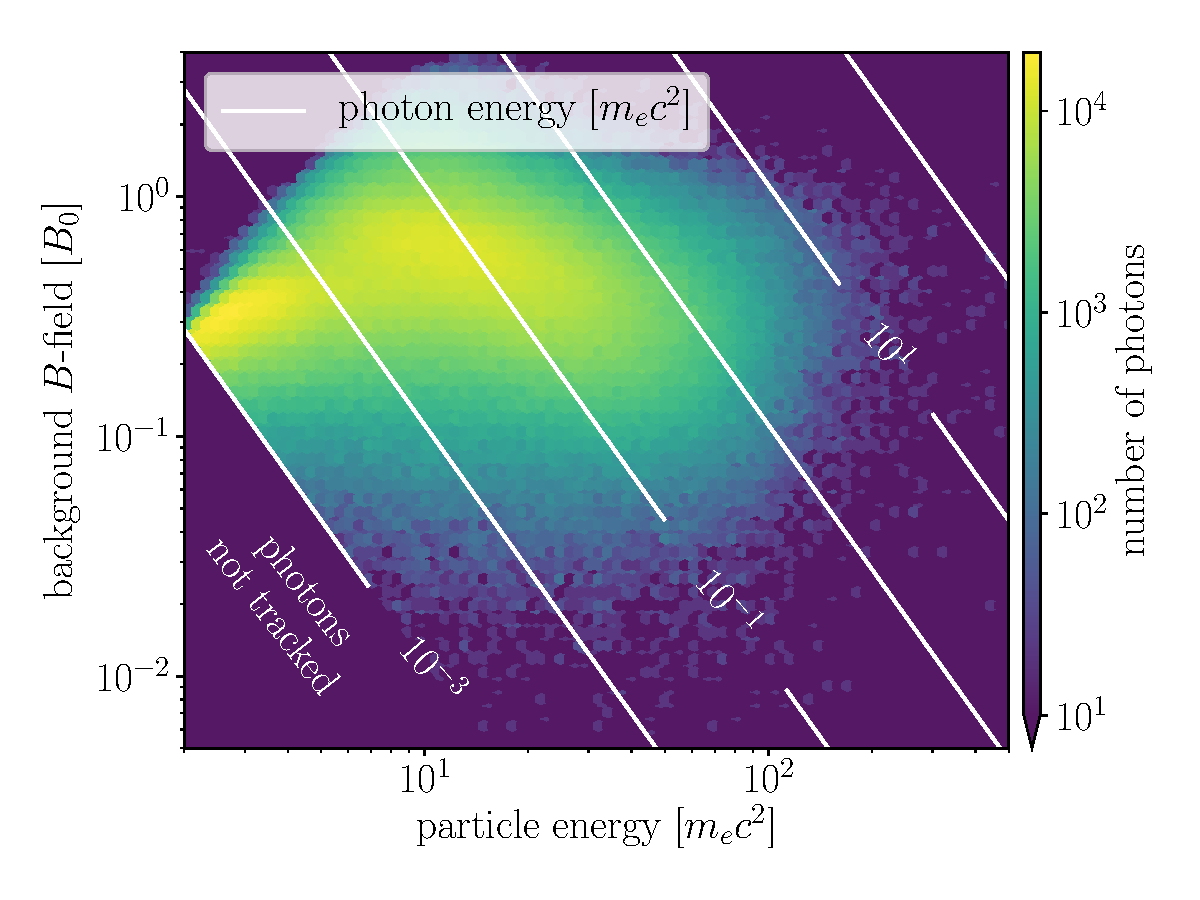
\includegraphics[width=0.5\textwidth]{figures/ch4-pairproduction/fig_b1.pdf}
    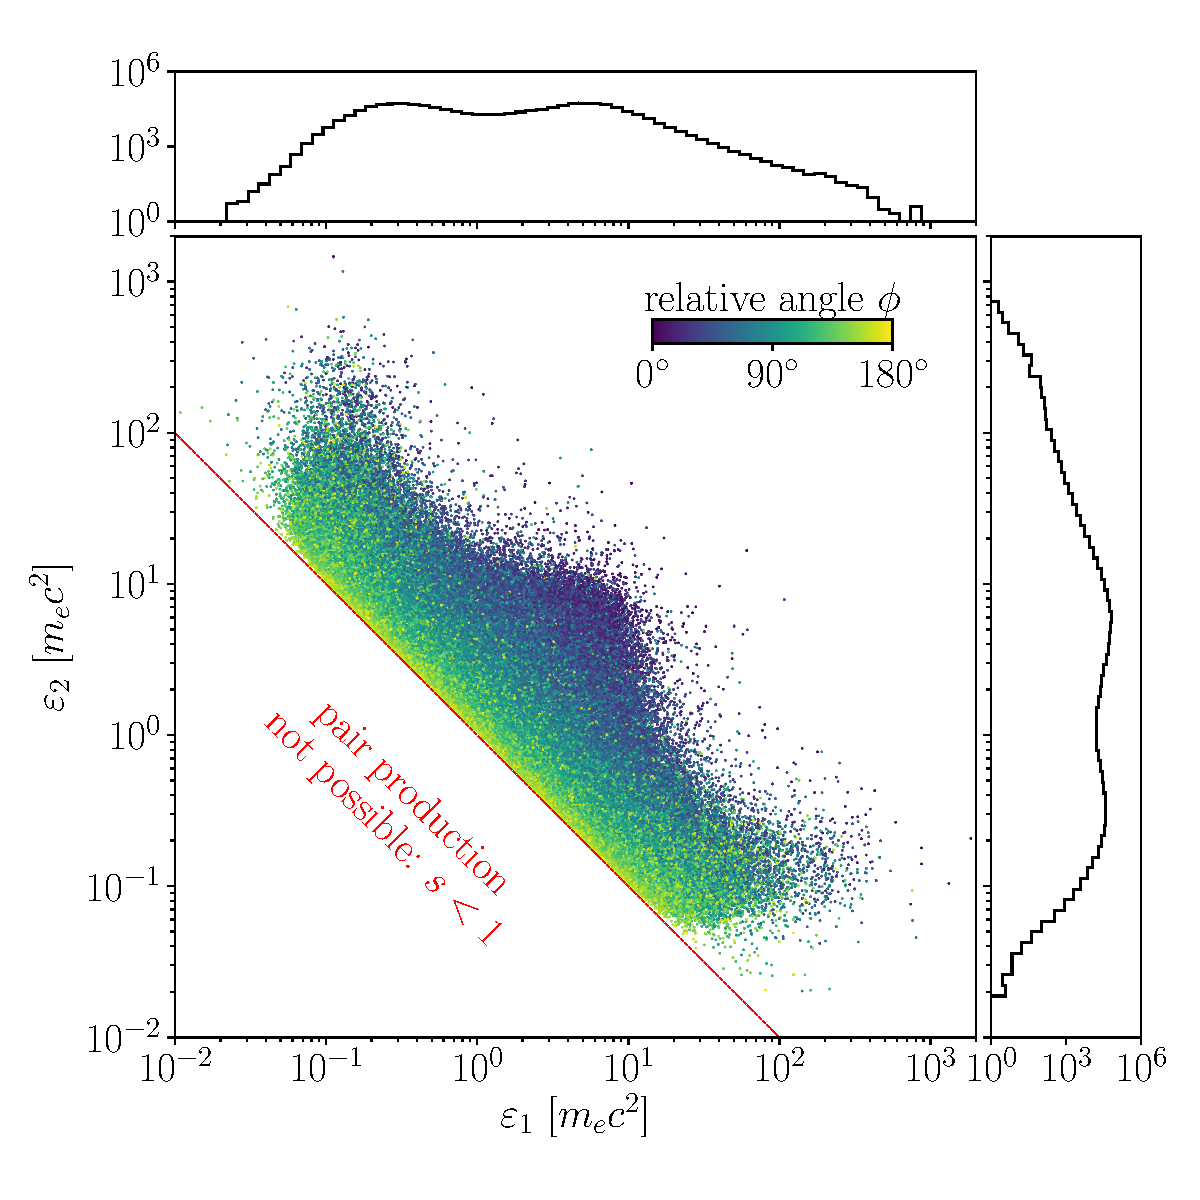
\includegraphics[width=0.4\textwidth]{figures/ch4-pairproduction/fig_b2.pdf}
    \caption{{\it Left:} 2D histogram of the radiated synchrotron photons vs the particle energy and the background magnetic field from one of our simulations ($\sigma_{\rm c}=5000$, $\gamma_c=50$, $\gamma_{\rm rad}=200$, $p_0=10^{-5}$). Each particle radiates at a corresponding synchrotron frequency (white contours), set by an effective background magnetic field (y-axis) and the Lorentz-factor of the particle (x-axis). Photons below $10^{-3}m_e c^2$ are not tracked, since they do not participate in pair production. {\it Right:} pair production statistics from the same simulation as on the left. Each point is a pair production event with $x$ and $y$ axes corresponding to the interacted photon energies and colors corresponding to their relative angles. One dimensional histograms are shown above and to the right, demonstrating that a wide range of photon energies are roughly equally important in terms of pair production.}
    \label{fig:pairprod-phot_born}
\end{figure}

Figure~\ref{fig:pairprod-phot_born} ({\it right}) shows the statistics of pair production from the same run, scatter plotted against the energies of two photons that produced the pairs. Each point is the pair production event, the color of each point represents the relative angle, $\phi$, between photon momenta. As one could have anticipated, the closer the energy product $\varepsilon_1\varepsilon_2$ to $2m_e c^2$, the closer the relative angle to $180^{\circ}$, and vice versa: two high energy photons can interact if their relative angle is small.

As one can also see from the one-dimensional histograms (Figure~\ref{fig:pairprod-phot_born}, {\it right}), the majority of pair production is for the photon energies $\varepsilon>10^{-2}m_e c^2$, and, thus, the photon tracking energy limit (which in this case is $10^{-3} m_e c^2$) is justified. Two extended scatter ``wings'' to the right and up are due to the fact that some very high energy photons do not have a low energy partner to interact (not tracked), and are left to interact with the higher energy ones. These tails, while being a numerical artifact, however, do not contribute much to pair production. We have carried convergence tests with lowering the energy limit with similar results: very low energy photons do not have a a significant contribution to pair production.

In Figure~\ref{fig:pairprod-energy_vs_time} the distribution of total energy in the box between different components is shown (normalized by the initial magnetic field energy, $U_B$). After the reconnection is triggered we let the initial plasma to escape through the boundaries perpendicular to the current sheet, which are being opened at around 1-2 light crossing times. After that new plasma (and thus magnetic flux) is injected at the boundaries, carrying additional energy, which is why we see that first spike in the plot. Most of the energy is carried by the magnetic field which in the process of regular reconnection is being transferred to primary generation of particles up to 2-3 box light-crossing times. At that point the synchrotron cooling and pair production are turned on and the reconnection relaxes to a new steady state.

At late times the energy is mostly contained in photons and secondary particles created in pair production events. The large ``waves" lasting a few box light-crossing times at late times are due to the large plasmoid, that constantly form, accumulate secondary plasma from the environment, and are then advected out from the box.

\begin{figure}[tb]
    \centering
    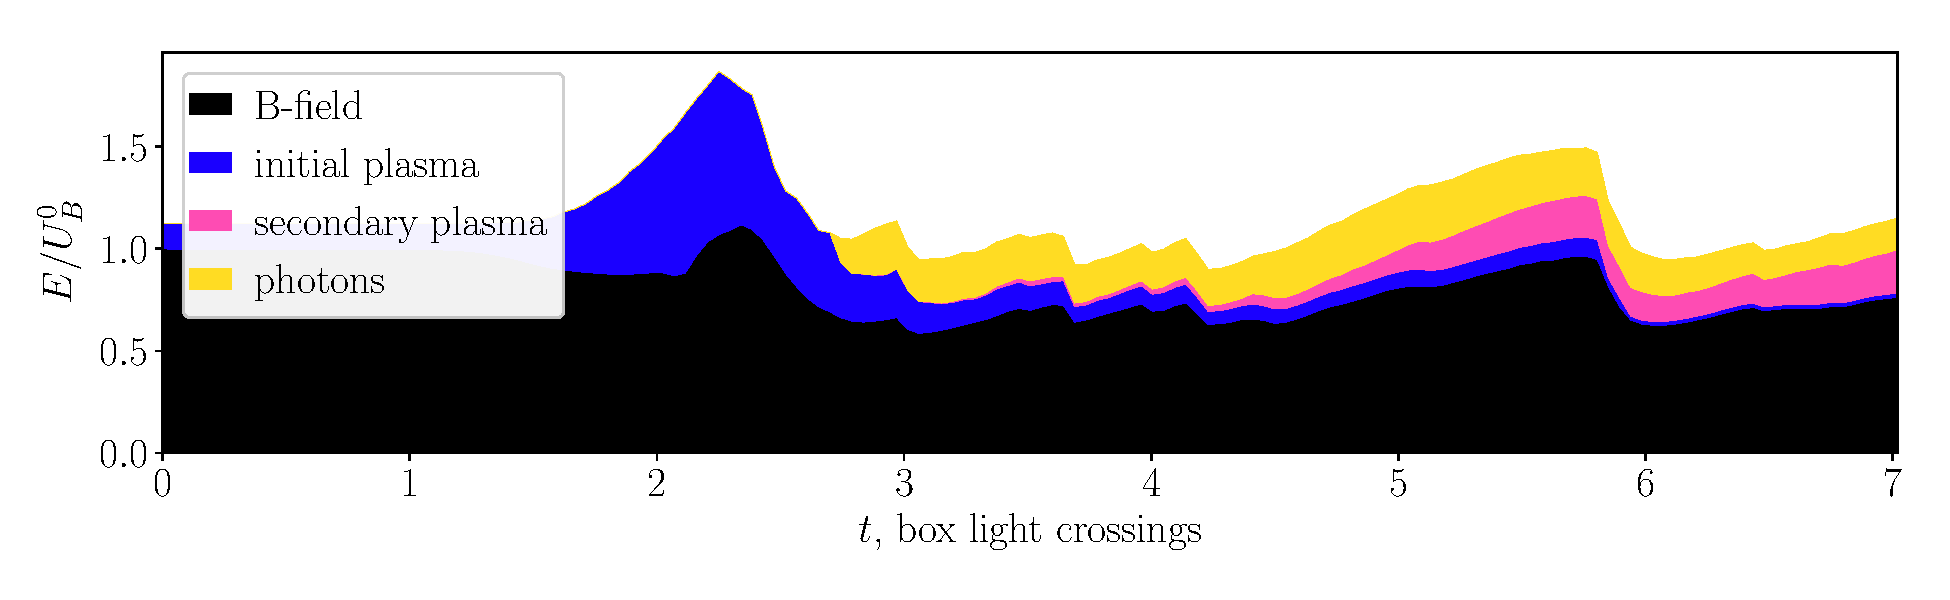
\includegraphics[width=0.9\textwidth]{figures/ch4-pairproduction/fig_b3.pdf}
    \caption{Energy partition in the simulation with $\sigma_{\rm c}=5000$, $\gamma_c=50$, $\gamma_{\rm rad}=1000$, $p_0=10^{-5}$. The energy is normalized by the initial magnetic field energy. Cooling and pair production is turned on at around three light-crossing times of the box. Large ``waves" are due to plasmoids forming, evolving and leaving the box in a few light-crossing times. One should keep in mind that the total energy of the magnetic field depends on the size of the region around the current sheet, and in this context it is rather artificial.}
    \label{fig:pairprod-energy_vs_time}
\end{figure}
